\documentclass[12pt]{article}
\usepackage{amssymb, amsmath, amsfonts, bm, graphicx, geometry}
\usepackage{tabularx, booktabs, float, enumitem, multicol, mathtools}
\geometry{margin=1in}


\title{}
\date{}
\author{}

\begin{document}

\begin{titlepage}
    \centering
    \vspace*{1in}

    % Title of the experiment and identifying number
    {\Large\bfseries Lab 3: Verification of the Maximum Power Transfer Principle \par}
    \vspace{1.5cm}

    % Course number
    {\large ESC 221 Basic Principles of Electrical Engineering \par}
    \vspace{2cm}

    % Author's name
    {\large \textbf{Author:} Zeshui Song \par}
    \vspace{0.5cm}

    % Names of other lab group members
    {\large \textbf{Lab Partners:}} \\
    Roy He, Phillip Joseph, Bella Im, and Kieran Cheng
    \vfill

    % Date on which the lab was performed
    {\large Date Performed: April 2, 2026 \par}
    \vspace{0.8cm}

    % Name of organization sponsoring the work
    {\large Cooper Union \par}

    \vspace*{1in}
\end{titlepage}
\newpage

\section*{I. Introduction, Experimental Method and Hypotheses}
\textbf{A. Introduction}\\\\
This experiment aims to verify the maximum power transfer principle, which states that maximum power is delivered to a load when the load resistance equals the Thevenin equivalent resistance of the source.\\\\
\textbf{B. Experimental Method}\\\\
A DC circuit was constructed with a fixed voltage source and a resistor network. A potentiometer was used as a variable load resistor to adjust the load resistance. The voltage and current were measured across the load resistor for varying resistance values from 500 $\Omega$ to 5000 $\Omega$ in increments of 250 $\Omega$. These measurements were used to calculate the power delivered to the load and identify the resistance value at which maximum power transfer occurs.\\\\
\textbf{C. Hypotheses}\\\\
Shown by calculations in the Appendix, the Thevenin equivalent resistance of the source is approximately 2.779 k$\Omega$. Therefore, it is hypothesized that maximum power transfer will occur when the load resistance is approximately equal 2.779 k$\Omega$ as shown in the theoretical plot of power vs. load resistance in Figure \ref{fig:PowerPlot}.
\begin{table}[h]
\centering
\begin{tabular}{cccc}
\hline
$R_{3}$ ($\Omega$) & $V_{3}$ (V) & $I_{3}$ (mA) & $P_{3}$ (mW) \\ \hline
500 & 1.08 & 2.16 & 2.34 \\
750 & 1.51 & 2.01 & 3.03 \\
1000 & 1.88 & 1.88 & 3.53 \\
1250 & 2.20 & 1.76 & 3.88 \\
1500 & 2.49 & 1.66 & 4.12 \\
1750 & 2.74 & 1.57 & 4.30 \\
2000 & 2.97 & 1.48 & 4.41 \\
2250 & 3.17 & 1.41 & 4.48 \\
2500 & 3.36 & 1.34 & 4.52 \\
2750 & 3.53 & 1.28 & 4.53 \\
3000 & 3.68 & 1.23 & 4.52 \\
3250 & 3.82 & 1.18 & 4.50 \\
3500 & 3.96 & 1.13 & 4.47 \\
3750 & 4.08 & 1.09 & 4.43 \\
4000 & 4.19 & 1.05 & 4.38 \\
4250 & 4.29 & 1.01 & 4.33 \\
4500 & 4.39 & 0.975 & 4.28 \\
4750 & 4.48 & 0.942 & 4.22 \\
5000 & 4.56 & 0.912 & 4.16 \\ \hline
\end{tabular}
\caption{Calculated power values for varying load resistance values.}
\label{tab:load_data_mw}
\end{table}
\newpage
\begin{figure}[H]
    \centering
    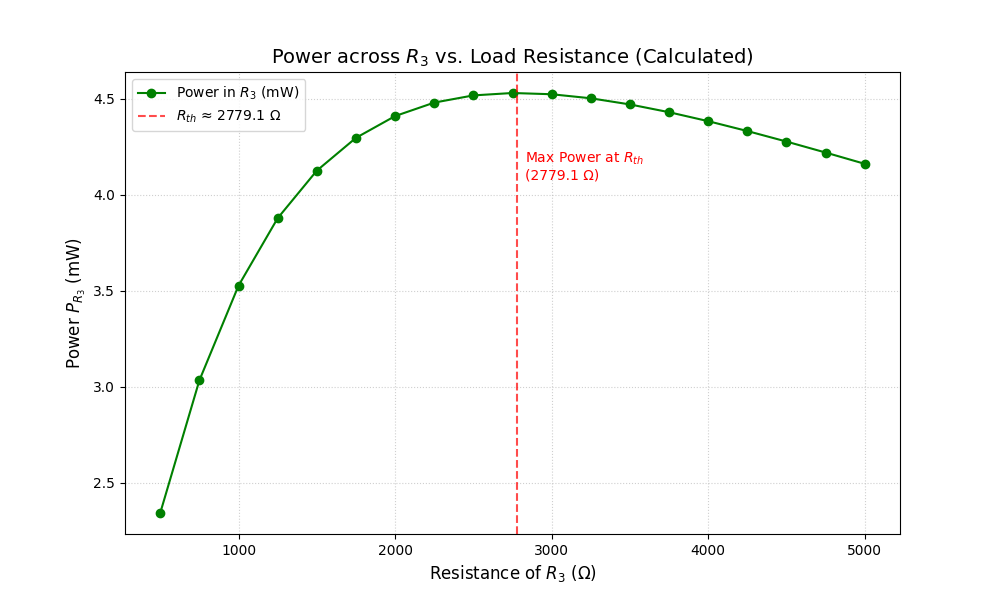
\includegraphics[width=1\linewidth]{Figure_1.png}
    \caption{Theoretical power delivered to the load resistor vs. load resistance with max power transfer occurring at $R_3 = R_{th}$.}
    \label{fig:PowerPlot}
\end{figure}\noindent
The plot of load voltage vs. load current ($V_{R_3}$ vs. $I_{R_3}$) is expected to show the following linear relationship as shown in Figure \ref{fig:VoltageCurrentPlot}:
\[V_\text{th} - I_{R_3} R_{th} - V_{R_3} = 0\quad\text{(KVL)}\]
\[V_{R_3} = V_\text{th} - I_{R_3} R_{th}\]
\[\implies \frac{\Delta V_{R_3}}{\Delta I_{R_3}} = -R_{th}\]
\begin{figure}[H]
    \centering
    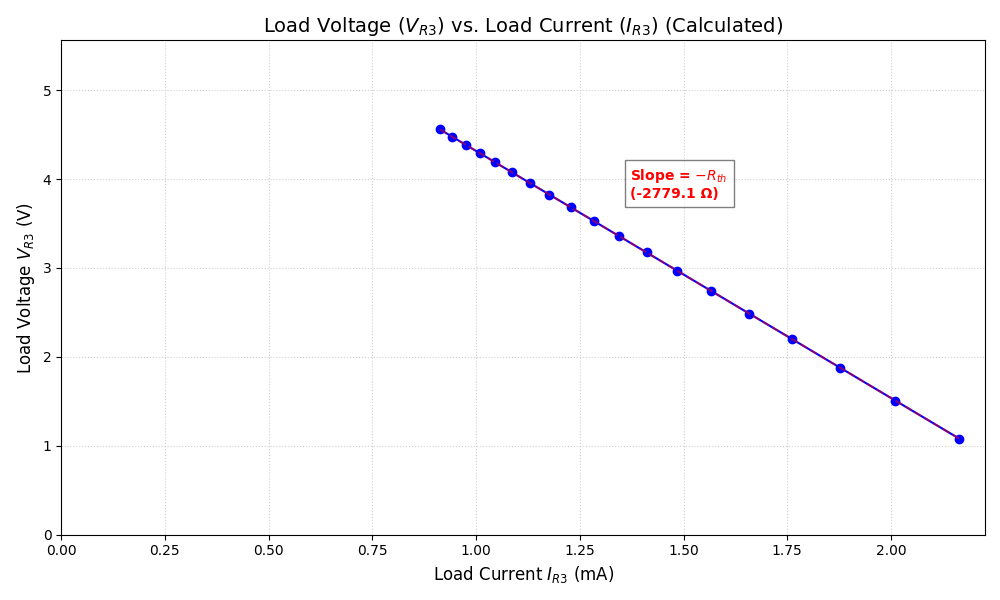
\includegraphics[width=1\linewidth]{Figure_2.png}
    \caption{Theoretical load voltage vs. load current with slope of magnitude equal to the Thevenin equivalent resistance $R_{th}$.}
    \label{fig:VoltageCurrentPlot}
\end{figure}\noindent\newpage
\section*{II. Equipment List}
\begin{enumerate}
    \item \textbf{Digital Multimeter} \\ 
          Manufacturer: AstroAI \\
          Model: AM33B
    \item \textbf{DC Power Supply} \\ 
          Manufacturer: GW Instek \\
          Model: SPD-3606
\end{enumerate}
\newpage
\section*{III. Wiring / Schematic Diagram / Procedure}
\textbf{A. Procedure}\\\\
1. Constructing the Circuit
\begin{enumerate}
    \item The circuit was constructed as shown in Figure \ref{fig:Circuit} with a fixed voltage source $v_1$ and resistors $R_1$ and $R_2$ with a variable load resistor $R_3$ connected across nodes a and b.
    \item A multimeter was connected in parallel across the load resistor $R_3$ to measure the voltage $V_{R_3}$ and resistance $R_3$.
    \item A multimeter was connected in series with the load resistor $R_3$ to measure the current $I_{R_3}$.
\end{enumerate}
2. Data Collection
\begin{enumerate}
    \item The load resistance $R_3$ was set to 500 $\Omega$ and confirmed using the multimeter.
    \item The voltage $V_{R_3}$ across the load resistor and the current $I_{R_3}$ through the load resistor were measured and recorded.
    \item Steps 1 and 2 were repeated for varying load resistance values from 500 $\Omega$ to 5000 $\Omega$ in increments of 250 $\Omega$.
\end{enumerate}
\textbf{B. Schematic Diagram}
\begin{figure}[H]
    \centering
    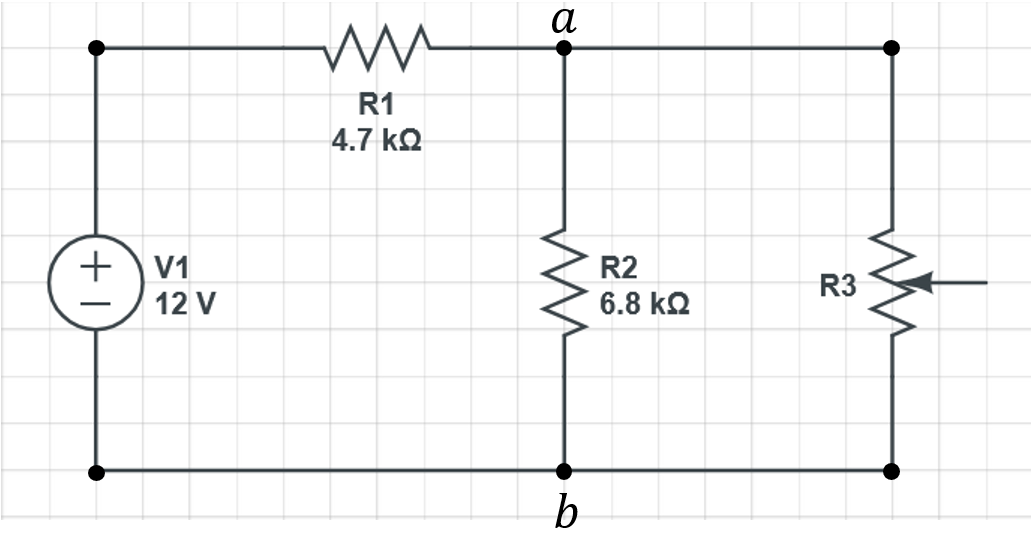
\includegraphics[width=0.6\linewidth]{Circuit.png}
    \caption{A DC circuit network consisting of a fixed voltage source $v_1$ and resistors $R_1$ and $R_2$ with a variable load resistor $R_L$ connected across the output. Nodes a and b are labeled for measurement points.}
    \label{fig:Circuit}
\end{figure}
\newpage
\section*{IV. Results}
\begin{table}[h]
\centering
\begin{tabular}{cccc}
\hline
$R_{3}$ ($\Omega$) & $V_{3}$ (V) & $I_{3}$ (mA) & $P_{3}$ (mW) \\ \hline
500 & 1.34 & 2.68 & 3.60 \\
750 & 1.85 & 2.46 & 4.54 \\
1000 & 2.28 & 2.28 & 5.19 \\
1250 & 2.65 & 2.12 & 5.62 \\
1500 & 2.97 & 1.98 & 5.89 \\
1750 & 3.25 & 1.86 & 6.07 \\
2000 & 3.50 & 1.75 & 6.12 \\
2250 & 3.72 & 1.65 & 6.15 \\
2500 & 3.91 & 1.57 & 6.12 \\
2750 & 4.09 & 1.49 & 6.07 \\
3000 & 4.24 & 1.41 & 5.99 \\
3250 & 4.38 & 1.35 & 5.89 \\
3500 & 4.50 & 1.29 & 5.79 \\
3750 & 4.61 & 1.23 & 5.67 \\
4000 & 4.71 & 1.18 & 5.55 \\
4250 & 4.80 & 1.13 & 5.42 \\
4500 & 4.88 & 1.08 & 5.29 \\
4750 & 4.95 & 1.04 & 5.16 \\
5000 & 5.02 & 1.00 & 5.04 \\ \hline
\end{tabular}
\caption{Measured power values for varying load resistance values.}
\label{tab:load_data_measured}
\end{table}
\begin{figure}[H]
    \centering
    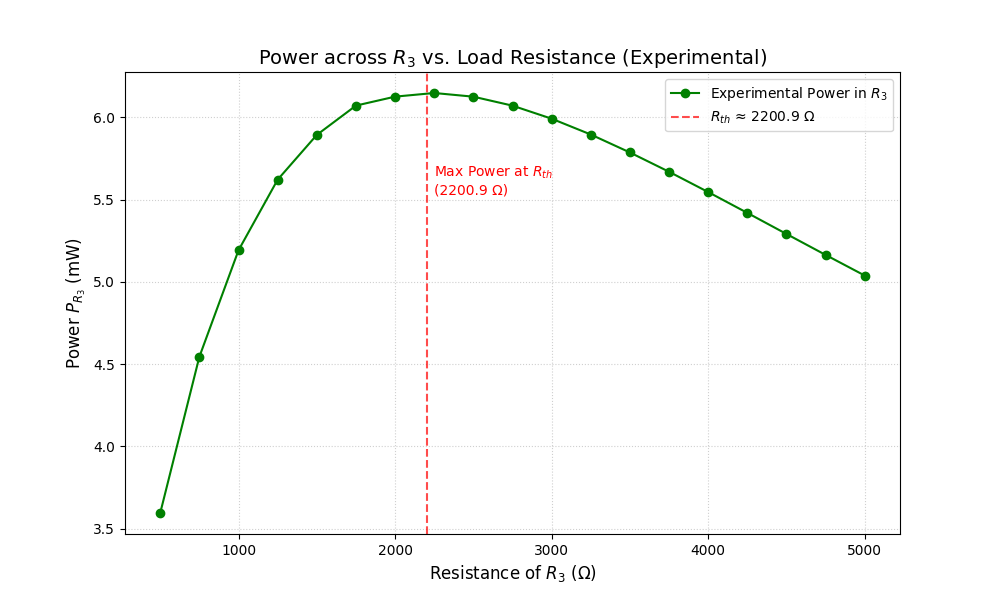
\includegraphics[width=1\linewidth]{Figure_3.png}
    \caption{The experimental power delivered to the load resistor vs. load resistance with max power transfer occurring at $R_3 \approx 2200.9\,\Omega$ (interpolated) which suggests that the actual resistor values for $R_1$ and $R_2$ differed from the theoretical values used.}
    \label{fig:exp1}
\end{figure}
\begin{figure}[H]
    \centering
    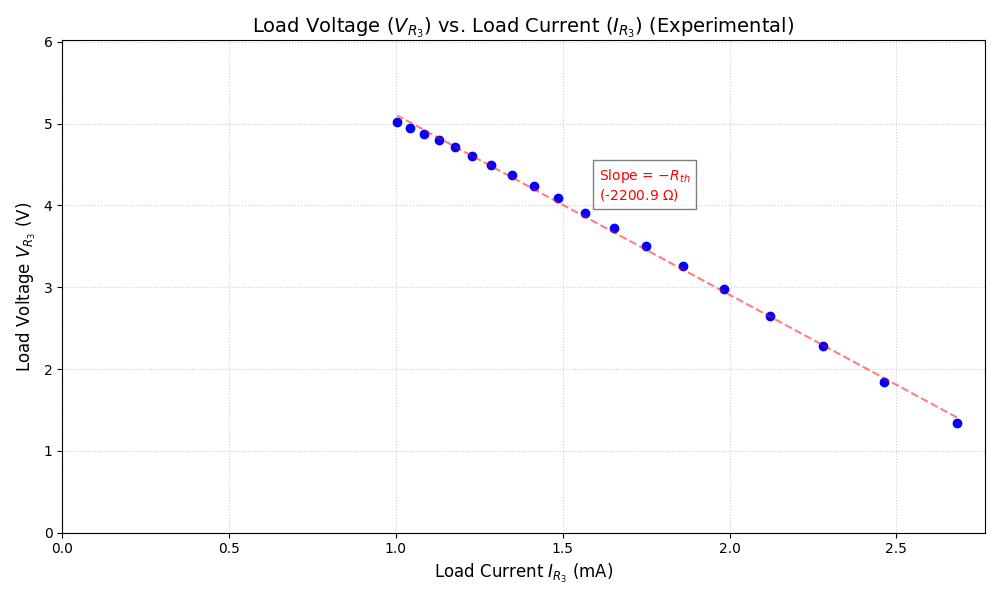
\includegraphics[width=1\linewidth]{Figure_4.png}
    \caption{The experimental load voltage vs. load current data is plotted in blue with a linear fit shown in red with slope of magnitude approximately equal to the experimental Thevenin equivalent resistance $R_{th}$.}
    \label{fig:exp2}
\end{figure}
\newpage
\section*{V. Discussion, Analysis and Concluding Statements}
\textbf{A. Slope of the load voltage vs. current plot}\\\\
The slope of the load voltage vs. current plot in Figure \ref{fig:exp2} is approximately equal to the negative of the Thevenin equivalent resistance $R_{th}$ of the source. This is consistent with the theoretical relationship derived from Kirchhoff's Voltage Law (KVL) which states that $V_{R_3} = V_\text{th} - I_{R_3} R_{th}$.\\\\
\textbf{B. Load resistance that had the max power dissipation}\\\\
The load resistance that had the maximum power dissipation was approximately 2200.9$\Omega$, which is closest to the $R_3=2250\,\Omega$ value as seen in Figure \ref{fig:exp1}. While close to the predicted value of 2779$\Omega$, this shows that the Thevenin equivalent resistance of the source was likely lower than the theoretical value calculated in the Appendix.\\\\
\textbf{C. Relationship to Thevenin equivalent resistance}\\\\
The maximum power transfer principle states that maximum power is delivered to the load when the load resistance equals the Thevenin equivalent resistance of the source. This is because we are able to redraw the circuit as a Thevenin equivalent circuit consisting of a Thevenin equivalent voltage source $V_\text{th}$ in series with $R_\text{th}$ and the load resistor $R_3$. Since current is equal in a series circuit, voltage division says that the max voltage across the load resistor $R_3$ occurs when $R_3 = R_\text{th}$. Thus, the maximum power delivered to the load occurs when $R_3 = R_\text{th}$.\\\\
\textbf{D. Conclusion}\\\\
This experiment verified the maximum power transfer principle, showing that maximum power was delivered when the load resistance approximately equaled the Thevenin equivalent resistance of the source. Although the experimental Thevenin resistance differed from the theoretical value, the strong linear relationship in Figure \ref{fig:exp2} indicates that this discrepancy likely arises from differences between the actual resistor values and those assumed in calculations.
\newpage
\section*{VI. Appendix}
\textbf{Calculations for Predicted Power Values}
\begin{center}
    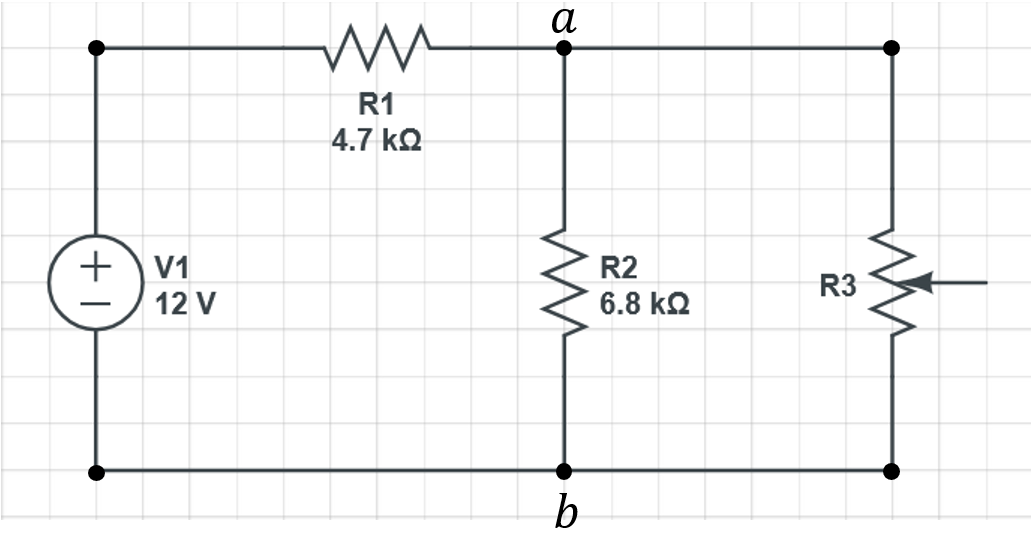
\includegraphics[width=0.6\linewidth]{Circuit.png}
\end{center}
To find the Thevenin equivalent resistance $R_{th}$ of the source, first remove the load resistor $R_3$ and turn off the voltage source $v_1$ (replace it with a short circuit). The remaining circuit consists of resistors $R_1$ and $R_2$ in parallel. Thus, the Thevenin equivalent resistance is given by:
\[R_{th} = \frac{R_1 R_2}{R_1 + R_2} = \frac{[4.7\,\text{k}\Omega]\cdot[6.8\,\text{k}\Omega]}{[4.7+6.8\,\text{k}\Omega]}=2.779\,\text{k}\Omega\]
\underline{Find the predicted voltage}\\
Find the Thevenin equivalent voltage $V_{th}$ by calculating the open-circuit voltage across nodes a and b. This can be done using voltage division:
\[V_{th} = v_1 \cdot \frac{R_2}{R_1 + R_2}= [12\,\text{V}]\cdot\frac{[6.8\,\text{k}\Omega]}{[4.7+6.8\,\text{k}\Omega]}=7.095\,\text{V}\] 
Using the Thevenin equivalent resistance, the circuit can be redrawn as a voltage source ($V_{th}$) in series with the Thevenin equivalent resistance ($R_{th}$) and the load resistor ($R_3$). Thus, the voltage across the load resistor $R_3$ can be calculated using voltage division:
\[V_{R_3} = V_{th} \cdot \frac{R_3}{R_{th} + R_3}\]
\underline{Find the predicted current}\\
The current through the load resistor $R_3$ can be calculated using Ohm's law:
\[I_{R_3} = \frac{V_\text{th}}{R_{th} + R_3}\]
\underline{Find the predicted power}\\
The power delivered to the load resistor $R_3$ can be calculated using the formula:
\[P_{R_3} = I_{R_3}^2 \cdot R_3\]
\end{document}